\chapter{Introduction}\label{chap:introduction}
\begin{chapabstract}

Intro intro intro intro.

\end{chapabstract}

\section{Star Formation Rate (SFR)}\label{sec:starformationrate}

Star formation in galaxies is one of the most complex processes.
In modern astronomy, understanding it and its evolution is still a challenging problem.
To explain these, we need an advanced knowledge of dark matter and baryon physics.
The evolution of dark matter is now interpreted by the ``$\Lambda$ CDM (Cold Dark Matter) model'' which indicates structures in the universe have been forming hierarchically (bottom-up) \citep[e.g.,][]{Peebles1982}.
This model explains that a galaxy forms in a small dark halo once and mergea into other halos to form larger systems as time goes on \citep{Blumenthal1984}.
With the advance of computational methods, a cosmological simulation can model this scenario and reproduce structures in the universe \citep[e.g.,][]{Navarro2000, Vale2004}.
However, the baryon evolution inside dark halos is much more difficult to understand because its evolution attributes to the composition of different scale of physics.
Revealing these physics needs as a first step to find constraints by measuring the star formation activity accurately.
When we measure the star formation activity at each era in the universe, we can constrain the galaxy evolution scenario observationally (Section~\ref{sec:cosmicstarformationhistory}).
The star formation rate (SFR) is the total mass of stars formed in a galaxy per year, and it is typically used for representing the star formation activity in a galaxy.
SFR is one of the most fundamental and important values for understanding galaxy properties and its evolution.

Here, we present the SFR calibration methods.
The fundamental equation to calculate SFR at time $t$ from intrinsic stellar luminosity at wavelength of $\lambda$ is shown below \citep{Buat1991}:

\begin{equation}\label{eq:Buat1991eq1}
    L\brp{\lambda,\,t}=\int_{0}^{t} \int_{\mr{M}\msb{low}}^{\mr{M}\msb{up}} F_{\lambda}\brp{m, \theta}\,\mr{SFR}\brp{t-\theta}\,\psi\brp{m}\,\mr{d}m \mr{d} \theta
\end{equation}
where $F_{\lambda}\brp{m, \theta}$ is the evolutionary stellar tracks, $\psi\brp{m}$ is the Initial Mass Function (IMF;~\citealt{Salpeter1955, Kroupa2001, Chabrier2003}) and $\mr{M}\msb{up}$ $\brp{\mr{M}\msb{low}}$ is the upper (lower) limit of the stellar mass considered for the calculation.

Indeed, we can calculate SFR from Equation~\ref{eq:Buat1991eq1} in two ways.
One way is to assume a certain stellar synthesis model and star formation history, and to calculate parameters to reproduce luminosities which we can observe at present.
This method is called SED fitting and it is useful even for the galaxies experienced not stable star formation recently.
However, this method highly depends on the star formation history chosen for the calculation.

Another way is to assume that $\mr{SFR}$ is constant over a certain timescale $T$ and SFR is proportional to the luminosity.
Although the timescale $T$ depends on the wavelength for measuring, it is simple to calculate SFR with a specific luminosity.
In this case, we can measure SFR with the following equation:

\begin{equation}\label{eq:Buat1991sfrproportion}
    \mr{SFR} = C \times L\brp{\lambda}
\end{equation}
where $C$ is a constant.

This method is relatively easy to measure SFR from an observation, but the assumption of a constant SFR is sometimes problematic.
Previous research show the required time to reach the steady state is $\sim\mr{Myr}$ for hydrogen recombination lines (e.g., $\mr{H\alpha};\,\lambda = 6563\,\mr{\AA}, \mr{H\beta};\,\lambda = 6563\,\mr{\AA}$), $\sim 100\,\mr{Myr}$ for the Far-ultraviolet (FUV) to IR emissions \citep{Hao2011, Murphy2011, Kennicutt2012}.
These result show that the SFR calculated from Equation~\ref{eq:Buat1991sfrproportion} is different from the true value if SFR varies among $\sim 10\,\mr{Myr}$ (e.g., Recent star burst).

Considering this problem, hydrogen recombination lines emitted by the young ($\leq 10^7\,\mr{yr}$) and massive ($M > 10\,M_{\odot}$) OB stars are more reliable SFR indicators.
However, in these cases, we should correct the dust extinction with the Balmer decrement which is the ratio between $\mr{H\alpha}$ and $\mr{H\beta}$ fluxes \citep{Lequeux1981}, or with IR luminosities \citep{Kennicutt2009}.
In addition to this, we need to eliminate [N\textsc{ii}] line contamination ($\lambda = 6548\,\mr{\AA}, 6584\,\mr{\AA}$) from $\mr{H}\alpha$ emission, and correct the absorption of $\mr{H\beta}$ by the young stellar atmosphere.
Although recombination lines are good SFR indicator in terms of the time scale in a constant star formation, the calibration for them gives us non-negligible uncertainty.

FUV emission is emitted by the A (or B) stars and it is reliable as SFR indicator if the star formation timescale can be assumed more than $10^8\,\mr{yr}$.
Because of its wavelength ({\it GALEX\/} FUV;\@$1516\,\mr{\AA}$), we need to correct the dust extinction also for FUV\@.
We often use IR luminosities for the dust correction based on the idea that dust grains absorbing FUV light re-emits it at a wavelength range of IR \citep{Kennicutt1998, Murphy2011}.
The combination of FUV and IR emissions for estimating SFR is one of the most popular SFR indicators (e.g., $\mr{FUV + 24mic}$, $\mr{FUV + total\,IR}$).

Besides these indicators, in this study, we focus on the low-frequency radio emission around\\ $\sim100\MHz$ because it is also a SFR indicator guaranteed by its correlated with (Far) IR emissions and SFR in galaxies (Section~\ref{sec:lowradiofrequenciesandsfr}).





\section{Cosmic Star Formation History}\label{sec:cosmicstarformationhistory}

\citet{Tinsley1980} proposed the cosmic star formation history which shows the SFR density evolution in the universe.
While no one could observe much more high-z galaxies enough to do the statistics at that time, we can now observe intrinsic FUV and IR luminosities from a large number of galaxies up to $z \sim 4$ (and up to $z \sim 7$ with only ultraviolet).
    Recent studies \citep{Hopkins2006, Madau2014} make a cosmic star formation history with a consistent IMF over all the redshift range.
Their plots represent that the peak of the star formation happened at $z\sim1.9$ where $3.5\,\mr{Gyr}$ after the Big Bang (Figure~\ref{fig:Madau2014_figure9}).
The era when the SFR density was the highest is called ``Cosmic Noon'' because the star formation in the universe was the most active.
The era before Cosmic Noon ($z > 1.9$) is called  ``Cosmic dawn''.

\begin{figure}[htbp]
	\centering
	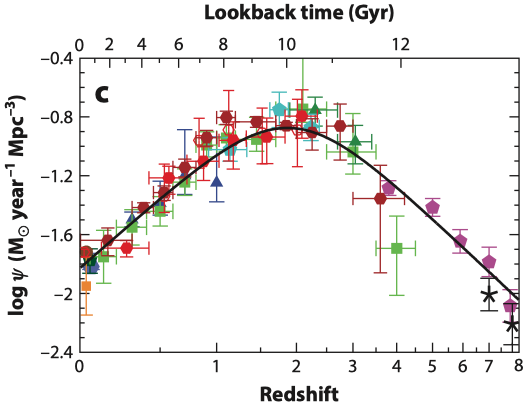
\includegraphics[width=.7\linewidth]{Chapter_1/Figures/Madau2014_Figure9.png}
    \caption[Reprint from \citet{Madau2014} (Figure~9)]{\label{fig:Madau2014_figure9}
        (Reprint from \citet{Madau2014}, Figure~9)\\
        This figure shows the cosmic star formation history from UV and IR emissions.
        For calculating SFR, they adopt Salpeter IMF\@.
        The black solid line shows the best fitting line.
        We can see the peak of SFR density in the universe at $z\sim1.9$
    }
\end{figure}

Although now we know the cosmic star formation history up to $z\sim8$ ($z > 4$ is still ambiguous due to the lack of IR observation), extending it to the earlier universe is quite difficult because we do not have a telescope to observe IR luminosity from high-z galaxies with a large field of view.
FUV emission from high-z galaxies is also difficult to be calibrated because the dust correction for high-z galaxies still have a large uncertainty.

On the contorary, the low-frequency emission is a extinction-free estimator and we will be able to observe high-z galaxies with a high sensitivity and large field of view enough to extend the cosmic star formation history.





\section{Low radio frequencies and SFR}\label{sec:lowradiofrequenciesandsfr}

The low-frequency radio emission from star-forming galaxies has been studied for many years.
In this paper, we use the term ``Low frequency'' as the frequency of a few $\GHz$ and less than that.
The importance of this emission increased after the global log-linear correlation with infrared (IR) had been found.
This correlation was discovered by \citet{Helou1985} using integrated far-infrared (FIR;\@$60\,\micron$ and $100\,\micron$) and $1.4\GHz$ radio luminosities in star-forming galaxies (Figure~\ref{fig:Helou1985_figure2}).
Although this correlation is originally called FIR-Radio Correlation, we use the term ``IR-Radio Correlation (IRC)'' because we tend to examine the correlation of radio with the total IR luminosity instead of FIR after \citet{Bell2003}.

\begin{figure}[htbp]
	\centering
	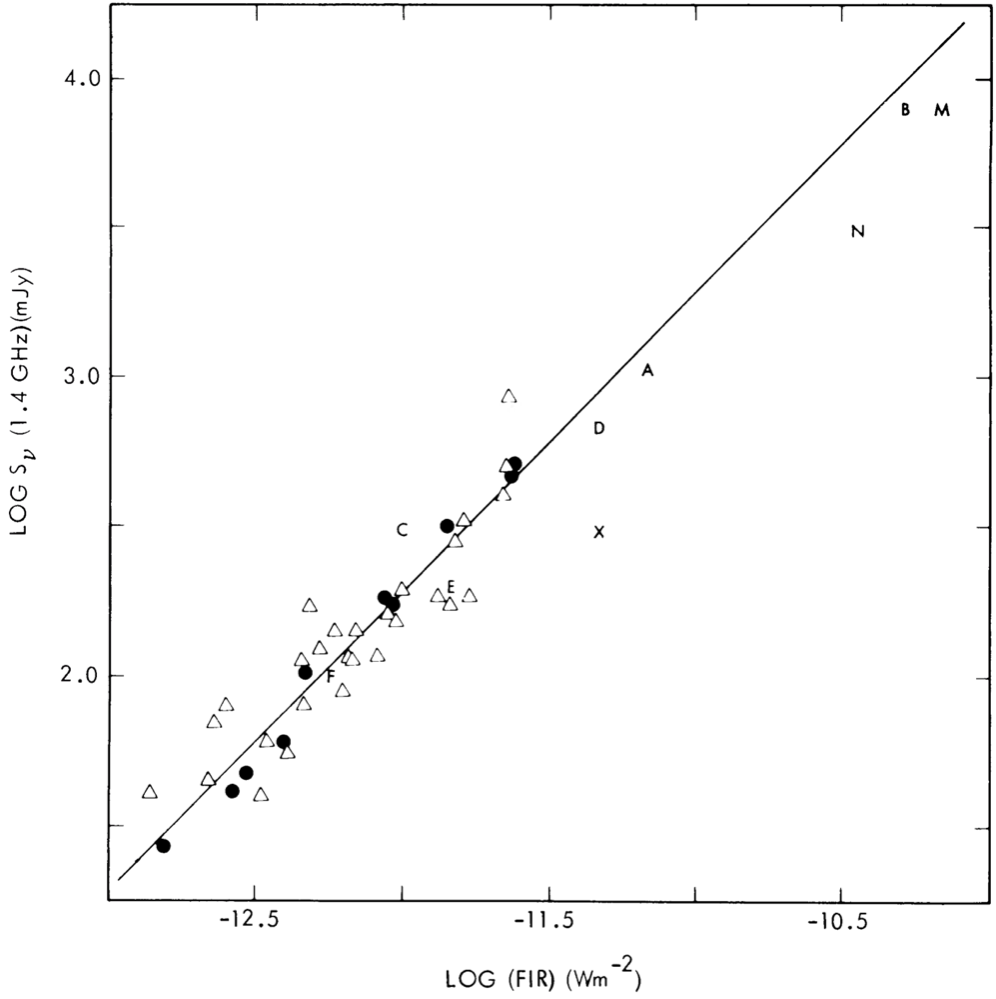
\includegraphics[width=.6\linewidth]{Chapter_1/Figures/Helou1985_Figure2.png}
    \caption[Adapted from \citet{Helou1985} (Figure~2)]{\label{fig:Helou1985_figure2}
        (Adapted from \citet{Helou1985}, Figure~2)\\
        This figure shows the comparison between FIR and radio at $1.4\GHz$ fluxes for each galaxy.
        We can see the tight correlation between them.
    }
\end{figure}

\citet{Condon1991a,Yun2001a, Bell2003} have examined this global correlation using a different sample set and found it holds the tightness across more than three orders of magnitude.
Recently, the low-frequency survey at around $100\MHz$ was operated by the LOw Frequency Array (LOFAR;~\citealt{VanHaarlem2013}) and the Murchison Widefield Array (MWA;~\citealt{Tingay2013a}).
With the advent of these telescopes, \citet{CalistroRivera2017a, Read2018, Wang2019} extend the study to at an order of magnitude lower frequency and find the correlation is held at not only $1.4\GHz$ but also $\sim 100\MHz$.
Thanks to this correlation, we can regard the low frequency emission as a SFR indicator because IR luminosity is emitted by heated dust grains in a galaxy and can measure the SFR\@.
Since the low-frequency emission is not affected by the dust extinction \citep{Yun2001a, Murphy2011} and it will be observed from a distant galaxies by the future extended survey, we anticipate its usefulness and need a further investigation of the relation between the radio and IR luminosities, especially its frequency dependence.

% Write a Calorimeter model
To explain IRC physically, \citet{Volk1989} proposed ``the calorimeter model''.
This model says that all energies from high energy electrons consumed before they escaping from galaxies is linearly correlated with all energies re-radiated as IR emissions by dust absorbing all FUV emission from young stars.

However, the spatially-resolved studies show that a star-forming galaxy emits the radio emission whose spectral index depends on the galaxy region \citep{Kapinska2017a, For2018a, Heesen2019} (Figure~\ref{fig:Kapinska2017_Figure5} and~\ref{fig:For2018_Figure6}).
This means that the radio emission is sensitive to the local density environment of the ISM and it is not guaranteed a simple frequency dependence of the global relation between the integrated radio and IR luminosities.

\begin{figure}[htbp]
	\centering
	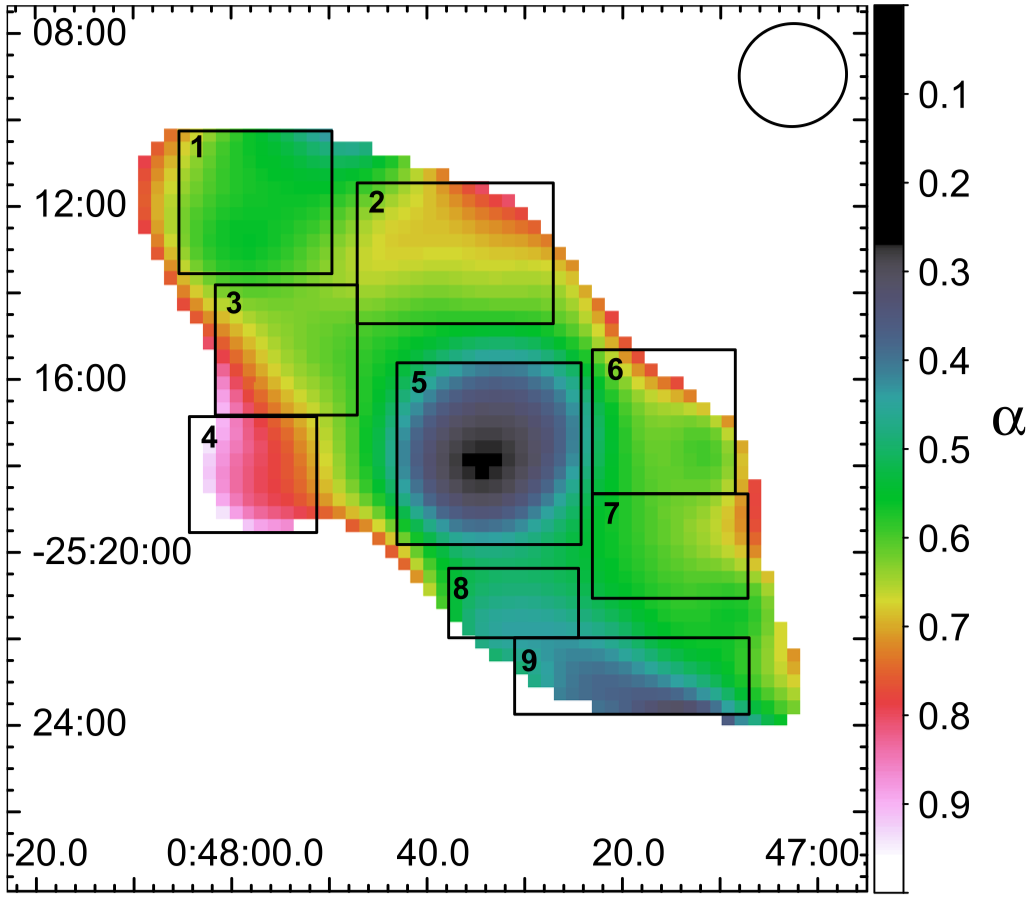
\includegraphics[width=.6\linewidth]{Chapter_1/Figures/Kapinska2017_Figure5.png}
    \caption[Adaptedfrom \citet{Kapinska2017a} (Figure~5)]{\label{fig:Kapinska2017_Figure5}
        (Adapted from \citet{Kapinska2017a}, Figure~5)\\
        This figure shows the distribution of the radio spectral index in NGC 253.
        They do the fitting between $200\MHz$ (GLEAM;\@\citealt{Hurley-Walker2017a}) and $1.465\GHz$ \citep{Carilli1992}.
        The color scale is for the spectral index and the pixel size is $18 \times 18 \arcs^2$.
    }
\end{figure}

\begin{figure}[htbp]
	\centering
	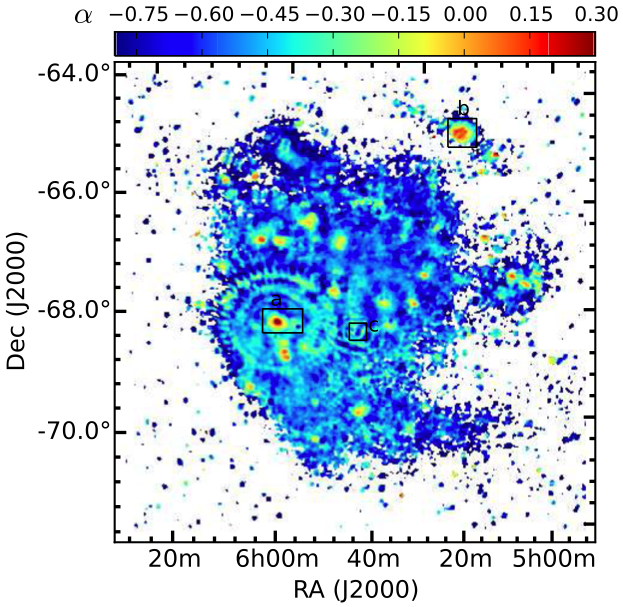
\includegraphics[width=.6\linewidth]{Chapter_1/Figures/For2018_Figure6.png}
    \caption[Adapted from \citet{For2018a} (Figure~6)]{\label{fig:For2018_Figure6}
        (Adapted from \citet{For2018a}, Figure~6)\\
        This figure shows the distribution of the radio spectral index in Large Magellanic Could (LMC).
        They do the fitting between $166\MHz$ (GLEAM;\@\citealt{Hurley-Walker2017a}) and $1.4\GHz$ \citep{Hughes2007}.
        The color scale is for the spectral index and the pixel size is $34.9 \times 34.9 \arcs^2$ at GLEAM 166MHz.
    }
\end{figure}

The integrated radio emission in star-forming galaxies across $100\MHz$ to $1.4\GHz$ is supposed to compose of a few percent to $10\%$ free-free and the synchrotron radiations \citep{Condon1992a}.
Each radiation is emitted by electrons interacted with the electric field of ions in the \ih~region or the magnetic field in a galaxy.
For emitting the synchrotron radiation, an electron needs to be accelerated to the light speed by the supernova remnant.
While the synchrotron emission is expected to be dominant at these low frequencies, previous studies find the sign of the free-free absorption and flatter or turnover spectral \citep{Schober2017, Chyzy2018}.
If the radio emission has a significant turnover among low frequencies, IRC does not have a simple frequency dependence and the radio emission is no longer useful as a SFR indicator.

In this study, we investigate nearby star-forming galaxies from the reference sample for ensuring the reliability of measuring the SFR from the low-frequency emission.
For examining the general trend, we use star-forming galaxy samples from Herschel Reference Survey (HRS;~\citealt{Boselli2010}) catalog which are supposed to represent the galaxy samples and the low-frequency emission from The GaLactic Extragalactic All-sky MWA (GLEAM;~\citealt{Hurley-Walker2017a}) Survey which observes the mJy scale radio emission from large areas with their 20 narrow bands.

This paper is organized as follows.
In Chapter~\ref{chap:data}, we introduce our galaxy samples and the low-frequency emissions used in this study.
In Chapter~\ref{chap:mmthod}, we introduce the IR-Radio Correlation with the $\qn$ value defined for evaluating the correlation quantitatively. Here, we also mention the way to investigate its frequency dependence and derive the radio SFR\@.
In Chapter~\ref{chap:results}, we show our results about the frequency dependence of IRC and the consistency of the radio SFR\@.
In Chapter~\ref{chap:discussions}, we compare our results with previous studies.
Finally, we summarize our study in Chapter~\ref{chap:summary}.



%\bibliographystyle{mnras}
%%\bibliography{example} % if your bibtex file is called example.bib
%\bibliography{masterthesis}




%Reference Table \ref{tab:Table1}.  And blah blah blah.
%
%\begin{table}[t]
%\caption[TOC Table Description]{Caption.}
%	\centering
%	\begin{tabular}{lcc}
%		\hline
%        {\textbf{Setting}}                      & \multicolumn{2}{c}{\textbf{Mt C/y}} \\
%		                                                           &         Min          &     Max      \\ \hline
%		AAA                         &          40          &      66      \\
%		BBB                               &          14          &      66      \\
%		CCC                                       &          18          &      43      \\
%		DDD      &          4           &    $>$12     \\
%		EEE                                  &          0           &      47      \\
%		FFF                    & 1$ \times $10$^{-4}$ &      52      \\
%		GGG &          8           &      42      \\ \hline
%	\end{tabular}
%    \label{tab:Table1}
%\end{table}
%
%\section{Figures}
%Reference Figure~\ref{fig:Fig1}.
%
%\subsection{This is a subsection}
%\begin{figure}[t]
%	\centering
%	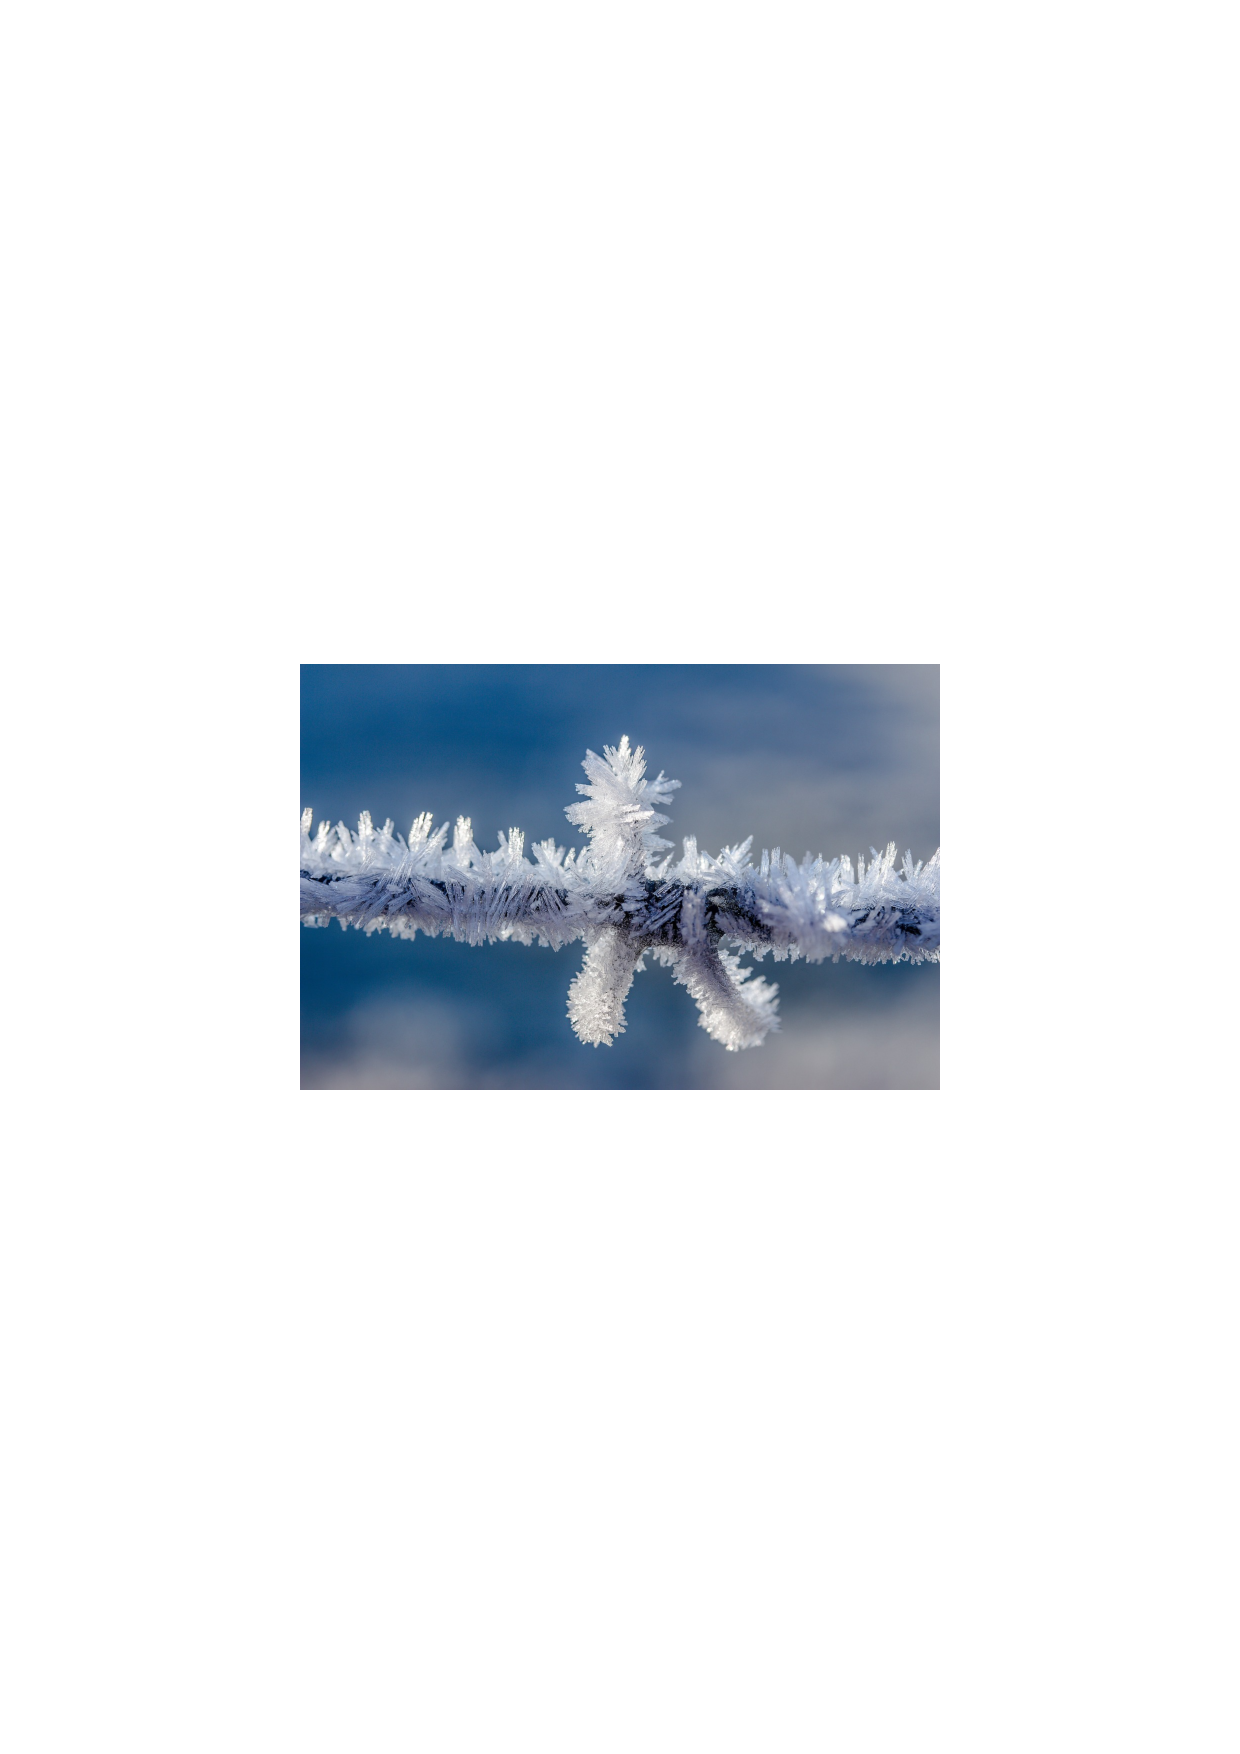
\includegraphics[width=.6\linewidth]{sFigs/Fig1.pdf}
%	\caption[TOC Figure Description]{Caption.}
%	\label{fig:Fig1}
%\end{figure}
%\subsubsection{This is a subsubsection}
%Citations are like \cite{goossens93,AbedonHymanThomas2003}.  Or maybe \cite{Abedon1994} said something.  Or \cite{Cerveny} which is an example of how to make a bib file that includes an author whose name begins with a non-English character and \cite{forgues96}: an example of referencing a Ph.D. thesis and yet more non-English characters.




%\bibliographystyle{abbrvnat}
%\bibliography{Chapter_1/ref1}
